% ------------------------------------------------------
%
% SALT Phase I Proposal Template
%
% This templates uses the saltproposal document class.
% You will need the "framed" LaTeX package to use it.
%
% Please email salthelp@saao.ac.za if you
% have any questions about this template.
%
% ------------------------------------------------------

% Do not change these options
\documentclass[10pt]{saltproposal}

\usepackage{lmodern}
\usepackage[T1]{fontenc}

\usepackage{graphicx}
\usepackage{epstopdf}

\begin{document}
	% IMPORTANT:
	% You cannot use floating environments such as the figure or
	% table environment.
	% In order to see what details are expected in the various
	% sections, have a look at the PDF output.
	
	
	\ScientificRationale{
	{\it In the last few weeks, our team has used a Monte Carlo radiative transfer
code to show that accretion disk winds can have a profound impact on the optical spectra of Cataclysmic Variables (CVs). Here we propose a set of spectroscopic observations of three CVs, 
with our motivation for submitting past the deadline being due to the following key points:

\begin{itemize}
\item The results which have led to this proposal have been {\bf very} recently obtained.
\item Due to the brightness of the objects, the observations are extremely cheap; we estimate a combined total of 30 minutes for the three objects in question to obtain signal-to-noise ratios of 30+. 
\item The data will be made publicly available, and serve as something of an online `atlas' for the CV community.
\item The spectra are required because broadband, single epoch spectroscopy of the systems in question is not currently available to the required spectral resolution.
\end{itemize}
}
\bigskip



Cataclysmic variables are systems in which a white dwarf accretes matter from a donor
star via Roche-lobe overflow. In non-magnetic nova-like systems (NMNLs) this accretion
is mediated by an accretion disk which forms around the white dwarf, and emits in the optical
and ultraviolet. NMNLs act as the perfect laboratory for accretion physics 
and testing of the `simple' disk model proposed by Shakura \& Sunyaev (1972), with one
specific example being the testing of the predicted $T\propto R^{-3/4}$ temperature 
profile with eclipse mapping (Rutten, van
Paradijs \& Tinbergen 1992).
\bigskip
%% be more specific ''in many ways'' -> goes
%% mention T~R3/4 ratios, eclipse mapping? 'simple' disk


For over three decades, it has been known that winds emanating from the accretion disk
are important in shaping the ultraviolet spectra of CVs (Heap 1978), 
the most spectacular evidence being the P-Cygni like profiles of resonance lines such as 
C${\textsc {iv}}$ (see e.g. Cordova \& Mason 1982). 
However, the extent to which winds influence optical spectra is not known, and even their origin 
and driving mechanism remains unclear (Drew \& Proga 2000). 
Answering these questions has far reaching implications, as
disk winds are of astrophysical importance across many orders of magnitudes in mass.
They are proposed as an important mechanism for AGN feedback (Silk \& Rees 1998) and shaping 
the spectra of Quasars (Weymann et al. 1991), and understanding them is vital to test
unification of accreting objects.
%% more here. Why are winds important? far reaching implications, big picture

\bigskip
Our recent Monte Carlo radiative transfer simulations (Matthews et al., in prep) expand on the work of Long \& Knigge (2002) by incorporating line transfer techniques suggested by Lucy (2002, 2003). Excitingly, these improvements have enabled us to show that the same outflow models used to explain the ultraviolet features seen in CVs also have a significant impact on optical features. In particular, we find that recombination lines in Hydrogen and Helium can be produced by a disk wind, and the same wind geometry can `fill in' the Balmer absorption edge that has thus far been present in CV models (but not observations; see e.g. Knigge \& Drew 1997). An example synthesized spectrum can be seen in Figure 1.
%% show spectra

\bigskip
We propose a spectroscopic study of three classic high-state systems at different inclinations. {\bf RW Sextantis, IX Velorium} and {\bf UU Aquarii} are all simple disk CVs with high accretion rates, and hence also have potential for mass loss. At inclinations of $\sim30^\circ$, $\sim60^\circ$ and $\sim80^\circ$ respectively these three objects provide opportunities to probe spectra across the full range of viewing angles. 
%% why are observations needed? why do we need better spectra? Specifics.
%% why use SALT?

\bigskip
These observations are essential for validating our results and will provide a useful resource to the community. They are required because sufficient quality spectra of NMNLs at varying inclinations are not available, and SALT's spectral capabilities provide the perfect opportunity to observe these objects.
In symbiosis with our modeling, the analysis of these spectra will help us to draw conclusions about the nature of the Balmer jump, the recombination lines of H and He and the continuity between disk atmosphere and disk wind. This will provide answers of astrophysical importance from a relatively modest time investment, and will also result in prompt publication for maximum benefit to the community.
	}
	


	% Immediate objectives.
	\ImmediateObjectives{ 
	Our objective is to use the wide-band spectrum for direct comparison with our radiative transfer simulations. 
	By obtaining spectra at a variety of inclinations we will be able to test for the presence or otherwise 
	of a Balmer jump in emission or absorption, discover trends in line emission strengths and profile shapes
	across the Balmer series, and assess the Helium emission. Combined with our theoretical work, 
	this will provide a unique insight into how much the disk wind affects the optical spectra of CVs.
	}
	


    % Completion requirements.
    \CompletionRequirements {
        % Insert your data requirements for completing the proposal here.
        Broadband optical spectra, as described in the technical justification, for all three objects: RW Sextantis, IX Velorium 
        and UU Aquarii. 
    } 
	
	

	% Technical justification.
	\TechnicalJustification{
		% Insert your technical justification here.
		In their normal state, RW Sextantis, IX Velorium and UU Aquarii have optical V band magnitudes of 
		$9.9$, $9.0$ and $13.3$ respectively (Ritter \& Kolb 2003).
		We require ${\rm SNR} \geq 30$ for all objects, but fortunately this is easily achievable with
		time budgets still being dominated by overheads. In total, we estimate 198.3 seconds of 
		total time (exposure plus overheads) for UU Aqr, and ?? and ?? for RW Sex and IX Vel respectively.

		We will be using RSS in long slit mode. Will will use the pg2300 grating which 
		provides coverage from ??? to ??? with a high enough spectral resolution. 
		We suggest the following grating angles, to be repeated for {\bf each} observation

		\begin{itemize}
		\item Camera Station $60.25^\circ$, Grating angle $48.875^\circ$. Simulation file uuaqr\_blue.rsim.
		\item Camera Station $70.75^\circ$, Grating angle $29.375^\circ$. Simulation file uuaqr\_mid.rsim.
		\item Camera Station $85.0^\circ$, Grating angle $39.125^\circ$. Simulation file uuaqr\_mid2.rsim.
		\item Camera Station $98.5^\circ$, Grating angle $49.25^\circ$. Simulation file uuaqr\_red.rsim.
		\end{itemize}

		These grating settings provide coverage from $\lambda 3505\AA- \lambda 6949 \AA$.
		This set of observations has a combined exposure time of ?? and overheads of ?? leading to a total ?? of time, and obtains 
		${\rm SNR} \geq 30$ for all observations, and ${\rm SNR} \sim 100$ in the majority of cases.
		}
	
	

	% Role of the PI.
	\RoleOfPI{
	    The PI will liase with the Co-Is and SA.
		% Insert the role of the PI here.
	}

	% References.
	\References{
	\ReferencePair
	    {Cordova \& Mason, 1982, ApJ, 260, 716}
	    {Dhillon 1996, IAU Colloq. 158: 208, 3}
	\ReferencePair
        {Drew \& Proga 2000, NewA Rev., 44, 21}
	    {Knigge \& Drew 1997, ApJ, 486, 445}	
	\ReferencePair
	    {Long \& Knigge 2002, ApJ, 579, 725}
	    {Lucy 2002, A\&A, 384, 725}
	\ReferencePair
	    {Lucy 2003, A\&A, 403, 261}
	    {Matthews et al., in preparation}
	\ReferencePair
	    {Ritter \& Kolb 2003, A\&A, 404, 301}
	    {Rutten, van Paradijs \& Tinbergen 1992, A\&A, 260, 213}
	\ReferencePair
	    {Shakura \& Sunyaev 1973, A\&A, 24, 337}
	    {Silk \& Rees 1998, A\&A, 331, L1}
	\ReferencePair
	    {Weymann et al. 1991, ApJ, 373, 23}
	%\ReferencePair
	%	{Linnell et al. 2010, ApJ, 719, 271}  %% The Anomalous Accretion Disk of the Cataclysmic Variable RW Sextantis
	%	{Beurmann et al. 1992, A\&A, 256,433} %% Phase-resolved spectroscopy of the novalike cataclysmic variable RW Sextantis
										  %% inclination 28-40

	}
	
	
	\AdditionalFigures{
	    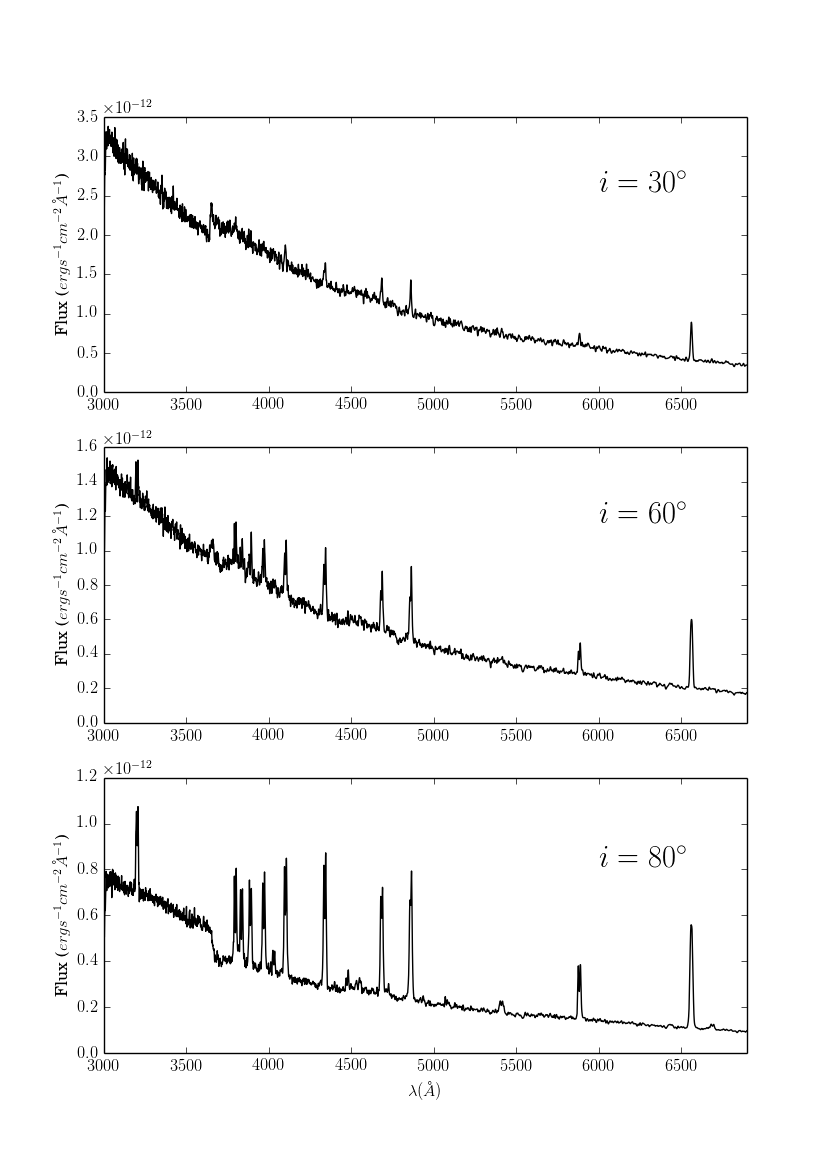
\includegraphics[height=300px]{specprop2.png}

	    \smallskip
	    {\bf Figure 1:} A simulated spectrum at angles of 30, 60 and 80 degrees, which are
	    the viewing angles corresponding showing to the inclinations of the three targets. 
	    Recombination lines in the Balmer series and Helium I \& II are prominent. The filling in
	    of the Balmer jump can be seen clearly in the highest inclination model. 
	    %caption{A simulated spectrum at angles of 30, 60 and 85 degrees showing clearly
	    %the recombination lines and lack of Balmer jump seen in our models.}
		% Insert any additional figures and graphics here.
		%
		% Allowable file types are:
		% If you are compiling using PDFLaTeX: JPG, PNG, PDF, EPS
		% If you are compiling with plain LaTeX: EPS only
		%
		% Example:
		% \includegraphics[height=200px]{Filename.eps}

	}

	
\end{document}
